\begin{figure}
\centering
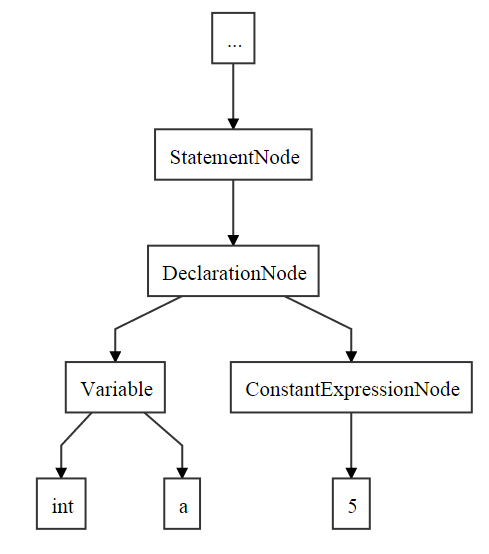
\includegraphics[width=0.5\textwidth]{figures/Trees/ASTAlone.PNG}
\caption{An \acrshort{ast} for the declaration \texttt{int a = 5;}}\label{fig:ASTAlone}
\end{figure}

\myref{fig:ASTAlone} shows a \texttt{DeclarationNode} for the expression \texttt{int a = 5;}. 
In the code generator this node will be transformed into the declaration written in C. 
The syntax for this is actually the same in C as it is in \gls{gamble}. 
The node has been through the previous phases, type and scope check, and is therefore ready to be computed.
The code executed when the visitor accepts a \texttt{DeclarationNode} can be seen on \myref{lst:DeclarationNodeCodeGen}.
\begin{lstlisting}[float, floatplacement=H!, caption=The visit method for visitting a DeclarationNode in the codegenerator. ,frame=tlrb,label={lst:DeclarationNodeCodeGen}]
@Override
public String VisitDeclarationNode(DeclarationNode node) {
    String expr = "";
    String complexType = "";
    if (node.getExpression() != null){
        resultVarStack.push(node.getVariable());
        expr = visit(node.getExpression());
        resultVarStack.pop();
    }

    if (node.getVariable().isComplex()) {
        ...
    }
    if (expr.indexOf("sclManageArgsLaunchKernel
    	(hardware, software, global_size, local_size") >= 0){
        ...
    }
    
    return complexType.length() > 0 ? complexType + expr : 
    (node.getVariable().toCcode() + " = " + expr + ";");
}
\end{lstlisting}
Since the example \texttt{int a = 5;} is not of a complex data type like a matrix or vector the body of the second and third if statements are hidden.\todo{Måske vise den i bilag hvor den ikke er hidden?}
A method is called on the node to check whether the expression that assigned the declared variable, exists. 
Syntactically a matrix or vector may appear to be uninitialised but this actually creates a vector or matrix filled with zeros.
In \myref{lst:DeclarationNodeCodeGen} the expression is not null so it enters the body of the \texttt{if} statement on line 5.
The result variable, which stores the result of the expression, is pushed to a stack before visiting the expression.
In the method \texttt{VisitExpresssionNode} the top of the stack, which the result was pushed to, is checked to see if the result is a complex datatype or not; in the example the result is not of a complex data type and the expression is then evaluated by visiting the nodes of the expression.
The result of the call to \texttt{VisitExpressionNode} is saved to a string \texttt{expr}.
Another if statement checks if the declaration needs a kernel and if the expression needs to be computed on the \acrshort{gpu}.
When the call to \texttt{VisitDeclarationNode} returns; a check is made if the string \texttt{complexType} has been made longer or not.
In the example \texttt{int a = 5;} it has not and therefore the string of the datatype and ID are concatenated with the assignment symbol, the substring \texttt{expr} and a semi-colon, before finally being returned.



